% GNUPLOT: LaTeX picture with Postscript
\begingroup
  \makeatletter
  \providecommand\color[2][]{%
    \GenericError{(gnuplot) \space\space\space\@spaces}{%
      Package color not loaded in conjunction with
      terminal option `colourtext'%
    }{See the gnuplot documentation for explanation.%
    }{Either use 'blacktext' in gnuplot or load the package
      color.sty in LaTeX.}%
    \renewcommand\color[2][]{}%
  }%
  \providecommand\includegraphics[2][]{%
    \GenericError{(gnuplot) \space\space\space\@spaces}{%
      Package graphicx or graphics not loaded%
    }{See the gnuplot documentation for explanation.%
    }{The gnuplot epslatex terminal needs graphicx.sty or graphics.sty.}%
    \renewcommand\includegraphics[2][]{}%
  }%
  \providecommand\rotatebox[2]{#2}%
  \@ifundefined{ifGPcolor}{%
    \newif\ifGPcolor
    \GPcolortrue
  }{}%
  \@ifundefined{ifGPblacktext}{%
    \newif\ifGPblacktext
    \GPblacktexttrue
  }{}%
  % define a \g@addto@macro without @ in the name:
  \let\gplgaddtomacro\g@addto@macro
  % define empty templates for all commands taking text:
  \gdef\gplbacktext{}%
  \gdef\gplfronttext{}%
  \makeatother
  \ifGPblacktext
    % no textcolor at all
    \def\colorrgb#1{}%
    \def\colorgray#1{}%
  \else
    % gray or color?
    \ifGPcolor
      \def\colorrgb#1{\color[rgb]{#1}}%
      \def\colorgray#1{\color[gray]{#1}}%
      \expandafter\def\csname LTw\endcsname{\color{white}}%
      \expandafter\def\csname LTb\endcsname{\color{black}}%
      \expandafter\def\csname LTa\endcsname{\color{black}}%
      \expandafter\def\csname LT0\endcsname{\color[rgb]{1,0,0}}%
      \expandafter\def\csname LT1\endcsname{\color[rgb]{0,1,0}}%
      \expandafter\def\csname LT2\endcsname{\color[rgb]{0,0,1}}%
      \expandafter\def\csname LT3\endcsname{\color[rgb]{1,0,1}}%
      \expandafter\def\csname LT4\endcsname{\color[rgb]{0,1,1}}%
      \expandafter\def\csname LT5\endcsname{\color[rgb]{1,1,0}}%
      \expandafter\def\csname LT6\endcsname{\color[rgb]{0,0,0}}%
      \expandafter\def\csname LT7\endcsname{\color[rgb]{1,0.3,0}}%
      \expandafter\def\csname LT8\endcsname{\color[rgb]{0.5,0.5,0.5}}%
    \else
      % gray
      \def\colorrgb#1{\color{black}}%
      \def\colorgray#1{\color[gray]{#1}}%
      \expandafter\def\csname LTw\endcsname{\color{white}}%
      \expandafter\def\csname LTb\endcsname{\color{black}}%
      \expandafter\def\csname LTa\endcsname{\color{black}}%
      \expandafter\def\csname LT0\endcsname{\color{black}}%
      \expandafter\def\csname LT1\endcsname{\color{black}}%
      \expandafter\def\csname LT2\endcsname{\color{black}}%
      \expandafter\def\csname LT3\endcsname{\color{black}}%
      \expandafter\def\csname LT4\endcsname{\color{black}}%
      \expandafter\def\csname LT5\endcsname{\color{black}}%
      \expandafter\def\csname LT6\endcsname{\color{black}}%
      \expandafter\def\csname LT7\endcsname{\color{black}}%
      \expandafter\def\csname LT8\endcsname{\color{black}}%
    \fi
  \fi
  \setlength{\unitlength}{0.0500bp}%
  \begin{picture}(7488.00,4464.00)%
    \gplgaddtomacro\gplbacktext{%
      \csname LTb\endcsname%
      \put(880,512){\makebox(0,0)[r]{\strut{} 0}}%
      \put(880,841){\makebox(0,0)[r]{\strut{} 2000}}%
      \put(880,1170){\makebox(0,0)[r]{\strut{} 4000}}%
      \put(880,1498){\makebox(0,0)[r]{\strut{} 6000}}%
      \put(880,1827){\makebox(0,0)[r]{\strut{} 8000}}%
      \put(880,2156){\makebox(0,0)[r]{\strut{} 10000}}%
      \put(880,2485){\makebox(0,0)[r]{\strut{} 12000}}%
      \put(880,2813){\makebox(0,0)[r]{\strut{} 14000}}%
      \put(880,3142){\makebox(0,0)[r]{\strut{} 16000}}%
      \put(880,3471){\makebox(0,0)[r]{\strut{} 18000}}%
      \put(976,352){\makebox(0,0){\strut{} 0.2}}%
      \put(1667,352){\makebox(0,0){\strut{} 0.4}}%
      \put(2359,352){\makebox(0,0){\strut{} 0.6}}%
      \put(3050,352){\makebox(0,0){\strut{} 0.8}}%
      \put(3742,352){\makebox(0,0){\strut{} 1}}%
      \put(4433,352){\makebox(0,0){\strut{} 1.2}}%
      \put(5125,352){\makebox(0,0){\strut{} 1.4}}%
      \put(5816,352){\makebox(0,0){\strut{} 1.6}}%
      \put(6508,352){\makebox(0,0){\strut{} 1.8}}%
      \put(7199,352){\makebox(0,0){\strut{} 2}}%
      \put(128,1991){\rotatebox{-270}{\makebox(0,0){\strut{}Wall Time ($\mu s$)}}}%
      \put(4087,112){\makebox(0,0){\strut{}Block Size (number of pages)}}%
    }%
    \gplgaddtomacro\gplfronttext{%
      \csname LTb\endcsname%
      \put(6560,4321){\makebox(0,0)[r]{\strut{}Naive, $mr\hat{\sigma}=$ 1.89 $avg\hat{\sigma}=$ 1.13}}%
      \csname LTb\endcsname%
      \put(6560,4161){\makebox(0,0)[r]{\strut{}Preallocated, $mr\hat{\sigma}=$ 3.19 $avg\hat{\sigma}=$ 1.73}}%
      \csname LTb\endcsname%
      \put(6560,4001){\makebox(0,0)[r]{\strut{}UnalignedNaive, $mr\hat{\sigma}=$ 8.45 $avg\hat{\sigma}=$ 2.10}}%
      \csname LTb\endcsname%
      \put(6560,3841){\makebox(0,0)[r]{\strut{}UnalignedPreallocated, $mr\hat{\sigma}=$ 2.59 $avg\hat{\sigma}=$ 1.88}}%
    }%
    \gplbacktext
    \put(0,0){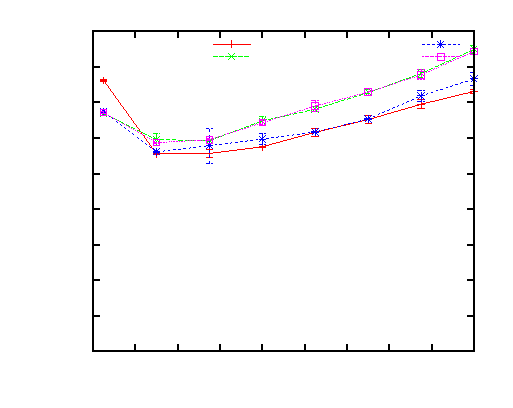
\includegraphics{PrecomputedRankBlockSize_Select_WallTime}}%
    \gplfronttext
  \end{picture}%
\endgroup
